\section{Benchmark Setup}
\label{sec:benchmark}

ACDB is organized around fixed benchmark instances rather than free-form causal-discovery episodes. Each instance defines a hidden causal world, a public data interface, and a benchmark-owned reference structure used later for scoring. This section makes that object concrete: what is sampled, what the agent sees, what remains hidden, and how accepted instances are assembled.

\paragraph{Task and instance family.} Each instance begins from a hidden linear-Gaussian structural causal model (SCM) over observed variables $X_1, \dots, X_d$:
\begin{equation}
X_i \;=\; \sum_{j \in \mathrm{Pa}(i)} w_{ij} X_j + \varepsilon_i,
\qquad \varepsilon_i \sim \mathcal{N}(0, \sigma_i^2),
\label{eq:linear-gaussian}
\end{equation}
where $\mathrm{Pa}(i)$ are the parents of $X_i$ in a directed acyclic graph (DAG) $G$ and the noise terms are jointly independent. The SCM induces an observational distribution $P(X)$ together with interventional distributions under hard single-node actions $\mathrm{do}(X_i = v)$, implemented by replacing the structural equation for $X_i$ with the assignment $X_i := v$ \citep{spirtes2000causation,eberhardt2005interventions}. Benchmark instances are therefore not abstract graph puzzles: they are sampled causal worlds that produce both an observational data matrix and intervention-specific sample matrices under the same underlying SCM.

Observational data do not generally identify a unique DAG. Distinct DAGs can share the same skeleton and the same v-structures, and are therefore Markov equivalent \citep{verma1990equivalence,andersson1997characterization}. ACDB represents this observational ceiling by the completed partially directed acyclic graph (CPDAG) of the instance. Directed CPDAG edges are compelled by the observational distribution, while undirected edges mark orientations that remain unresolved from $P(X)$ alone. The active task is therefore structured around two different causal objects (Figure~\ref{fig:dag-cpdag-intervention}): the CPDAG is the correct observational target, while the final submission target is a fully oriented DAG.

\begin{figure}[t]
\centering
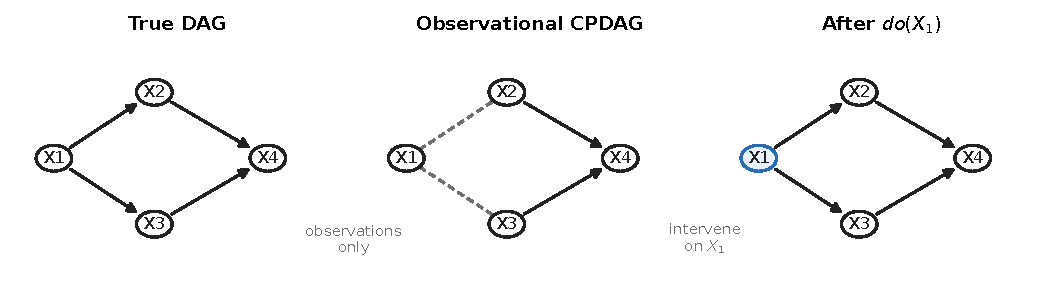
\includegraphics[width=\linewidth]{figures/generated/fig_dag_cpdag_intervention.pdf}
\caption{Observation identifies a CPDAG, not necessarily the full DAG. In this example the collider into $X_4$ is compelled from observational structure, while the two incident edges at $X_1$ remain undirected until an intervention on $X_1$ resolves them.}
\label{fig:dag-cpdag-intervention}
\vspace{-0.6em}
\end{figure}


\paragraph{Public runtime.} The agent interacts with each instance through a strict observe-intervene-submit protocol. The runtime releases the fixed observational sample $D^{\mathrm{obs}} \in \mathbb{R}^{n_{\mathrm{obs}} \times d}$ exactly once. After observation, the agent may spend a finite intervention budget on actions of the form $\texttt{intervene(var, value)}$, each of which returns a fresh sample matrix from the intervened SCM with shape $n_{\mathrm{int}} \times d$. Interventions are single-node and budgeted one call at a time; they are illegal before observation and impossible after the session is sealed. The episode terminates at $\texttt{submit\_graph}$, where the agent submits a mixed graph with directed and undirected edges. Allowing undirected submissions is deliberate: leaving an edge unresolved is a different outcome from omitting an adjacency or reversing a direction that should have been identified.

\paragraph{Accepted benchmark instance.} One accepted instance packages the tuple $\bigl(G,\; \mathrm{CPDAG}(G),\; \mathcal{S},\; \mathcal{I}^\star,\; D^{\mathrm{obs}},\; B,\; \pi \bigr)$, where $\mathcal{S}$ is the parameterized SCM, $\mathcal{I}^\star$ is a benchmark-owned minimum intervention set that resolves the CPDAG ambiguity for that world, $B = |\mathcal{I}^\star| + \texttt{budget\_slack}$ is the public intervention budget, and $\pi$ is a random permutation applied to anonymize node identities. Assembly is rejection sampling at three gates --- on the graph profile, on near-faithfulness of the parameterized SCM, and on the resolving-intervention profile (Algorithm~\ref{alg:instance-assembly}); predicate-level definitions of the gates are in Appendix~\ref{app:instance:filters}. The agent never sees $G$, $\mathrm{CPDAG}(G)$, $\mathcal{S}$, or $\mathcal{I}^\star$ directly: it sees only anonymized variable identities, the observational matrix, the remaining budget, and any interventional sample matrices returned by the runtime.

\begin{algorithm}[t]
\small
\caption{Accepted benchmark instance assembly. One iteration of the rejection loop draws a DAG, parameterizes a linear-Gaussian SCM, computes the resolving-intervention set, then permutes labels and samples the observational data. Three reject gates discard graphs with trivial CPDAGs, near-unfaithful SCMs, and CPDAGs that are already fully oriented. Predicate definitions are in Appendix~\ref{app:instance:filters}.}
\label{alg:instance-assembly}
\begin{algorithmic}[1]
\Require level config $(d,\; k,\; \texttt{weight\_range},\; \texttt{noise\_var},\; \texttt{faithfulness\_eps},\; n_{\mathrm{obs}},\; \texttt{budget\_slack})$; rng
\Ensure  accepted instance $(G,\; \mathrm{CPDAG}(G),\; \mathcal{S},\; \mathcal{I}^\star,\; D^{\mathrm{obs}},\; B,\; \pi)$
\Repeat
  \State $G \gets \texttt{sample\_random\_dag}(d, k;\; \mathrm{rng})$
  \State $C \gets \texttt{dag\_to\_cpdag}(G)$
  \If{$\texttt{reject\_graph}(G, C)$} \textbf{continue} \EndIf
  \State $\mathcal{S} \gets \texttt{parameterize\_linear\_gaussian\_scm}(G,\; \texttt{weight\_range},\; \texttt{noise\_var};\; \mathrm{rng})$
  \If{$\texttt{reject\_scm}(\mathcal{S},\; \texttt{faithfulness\_eps})$} \textbf{continue} \EndIf
  \State $\mathcal{I}^\star \gets \texttt{compute\_minimum\_intervention\_set}(G, C)$
  \If{$\texttt{reject\_intervention\_profile}(\mathcal{I}^\star, C)$} \textbf{continue} \EndIf
  \State $\pi \gets \texttt{random\_permutation}(d;\; \mathrm{rng})$
  \State relabel $(G,\; C,\; \mathcal{S},\; \mathcal{I}^\star)$ under $\pi$
  \State $D^{\mathrm{obs}} \gets \texttt{sample\_observational\_data}(\mathcal{S},\; n_{\mathrm{obs}};\; \mathrm{rng})$
  \State $B \gets |\mathcal{I}^\star| + \texttt{budget\_slack}$
  \State \Return $(G,\; C,\; \mathcal{S},\; \mathcal{I}^\star,\; D^{\mathrm{obs}},\; B,\; \pi)$
\Until{accepted}
\end{algorithmic}
\vspace{-0.4em}
\end{algorithm}

\paragraph{Benchmark family and assumptions.} The reported benchmark family is generated from level-specific configurations that vary graph size, edge count, observational and interventional sample counts, noise variance, and intervention slack while keeping the public interface fixed across levels. ACDB assumes full observability, causal sufficiency, and a linear-Gaussian SCM family. It also filters out near-unfaithful instances \citep{spirtes2000causation}, so accepted worlds do not sit arbitrarily close to vanishing partial correlations that would blur the intended observational structure at finite samples. Under these assumptions, classical constraint-based discovery is meaningful: with an exact independence oracle and enough data, PC recovers the true CPDAG, so finite-sample deviations can be interpreted as observational recovery error rather than latent-confounding error \citep{spirtes2000causation}. This is the benchmark setting within which the later score layers and ablations should be read.
